% para incluir python, las siguientes fuentes:
% https://ctan.org/pkg/pythontex
% https://tug.org/tug2013/slides/Mertz-A_Gentle_Introduction_to_PythonTeX.pdf
% https://www.12000.org/my_notes/python_in_latex/index.htm

%\chapterimage{chapter_head_1.pdf} % Chapter heading image
\chapter{Introducción}
\label{chap:intro}

\section{Motivación del proyecto}
\label{sec:resumen}
% # Resumen: Motivación del proyecto

El manejo de stock de terminales móviles es un gran desafío de logística para Antel,
que involucra varios proveedores, varios puntos de venta, 
y varios terminales (con una moda y obsolescencia bien marcada).
La falta de stock (\textit{stockout}) tiene un impacto en las compras de los clientes. 
Algunos clientes no compran un plan debido a la carencia del terminal deseado, 
y otros sustituyen el terminal por otro similar en stock. Este comportamiento determina que
no es correcto considerar el consumo de terminales igual a la demanda real.

\begin{remark}\textbf{El objetivo de este trabajo es estimar la demanda real de terminales, 
a partir del consumo realizado en cada punto de venta, 
estimando la falta de stock y el desistimiento o sustitución por parte del consumidor.}\end{remark} 

También se analiza la utilización real de terminales mediante datos de uso en la red,
y se compara la utilización con las ventas de terminales.
Para realizar el proyecto se utilizará información de estado de la red móvil y registros
de ventas de terminales. Esta información a mostrado ser imprescindible y suficiente
en modelos similares~\cite{Karabati2009, Letham:2016}. Se utilizará exclusivamente información ya disponible en
los sistemas informáticos manejados por los patrocinadores del proyecto. 
No se requiere información personal, y en caso de acceder a la misma será anonimizada\footnote{Datos \emph{anonimizados} significa que no se conoce (ni se puede inferir) la identidad de los usuarios. Utilizando un número opaco para identificar a cada usuario (sin significado en la realidad).}.

Para construir el modelo se utilizarán técnicas de aprendizaje automático y minería
de datos, aplicadas sobre grandes volúmenes de información (random forest, support vector machine, etc.). 
El responsable del proyecto cuenta con experiencia previa
en estas áreas de conocimiento  (\emph{machine learning,  data mininig, big-data}).


\section{Resumen ejecutivo}
\label{sec:ejecutivo}

\subsubsection{Sobre las fuentes de información.}
Se cuenta con registros de ventas de terminales desde mayo de 2014 a agosto de 2016, un total de
1.4MM de ventas realizada por Antel o agentes. 
Hay varios cambios de comportamiento en los datos; debido a promociones,
cambios de políticas en subsidios, cambio en los puntos de venta, etc. 
Por lo tanto, en la mayoría de este análisis eliminaremos estos efectos, 
y solo consideraremos las ventas en el período comprendido entre 01/12/2015 y 30/06/2016, que son $330k$ en total.

También se cuenta con logs del sistema EIR, quien registra los cambios de terminales asociados a cada contrato. 
Esto significa que solo se registra cuando un usuario cambia el chip desde un terminal a otro.
El resto de los eventos no se registra, siendo entonces una información muy valiosa pero parcial del uso de la red.
Se cuentan con datos de cambio de fidelidad en el período comprendido entre 31/08/2014 y 31/08/2016, 
que son 25MM de registros en total.
En el proceso de análisis se identificó que es necesario limpiar esta base de datos debido a inconsistencias que presentan los datos, 
y para algunos cálculos, como el uso efectivo de un terminal, es recomendable utilizar otra fuente de información, como ser el registro de llamadas/mensajes en la red móvil.

En Hadoop se dispone de información histórica reciente sobre las llamadas telefónica,
y la mensajería móvil (SMS). En este proyecto se utiliza esta información en el período del
25/01/2017 al 29/03/2017, período bastante alejado de la fecha de compra del terminal.
Esta información, junto a la información histórica sobre el número de cliente de Antel asociado
a un servicio móvil, es utilizada para medir el grado de cercanía entre dos usuarios del mismo terminal.

\subsubsection{Sobre los objetivos y resultados.}
Respecto a las ventas, 
es claro que unas pocas marcas y modelos de terminal concentran la mayoría de las ventas.
También hay diferencias marcadas entre los locales de Antel y los agentes, 
pero pocas diferencias entre locales de Antel. 
A modo de resumen, los agentes y Antel presentan distinto volumen de venta por local, 
siendo menos uniforme para locales de Antel. 
Los modelos de terminales vendidos difieren entre agentes y Antel.
La falta de stock también es distinta, siendo más frecuente en locales de Antel, 
sin mostrar grandes diferencias entre los principales locales de Antel y el resto.

Las ventas presentan una clara periodicidad semanal, pero no hay periodicidad según el día del mes, 
o la semana del mes donde se hace la compra.
Las ventas son en general muy irregulares en el tiempo, siendo un poco más homogéneas en los agentes
(son curvas más suaves, y más considerando que venden menos volumen). 
En los datos puede observarse fácilmente las fechas de comienzo y fin de la comercialización para algunos terminales, 
también la moda en el consumo, así como la carencia de stock por períodos extensos.

En el trabajo se estudia qué variables le importan al cliente al momento de elegir el nuevo terminal.
Para esto se evalúa la capacidad de predicción de cada variable en forma independiente y conjunta.
El mejor predictor encontrado tiene una exactitud de $58\%$, 
y utiliza exclusivamente las variables: plan del servicio, fecha de compra, tipo de local, y marca/modelo del terminal
anterior. Estas variables son sencillas de obtener al momento de la compra, y pueden guiar al
vendedor para ofrecerle al cliente algo a su medida. Así como también pueden ser incluidas en un
algoritmo recomendador para las ventas online.
Este predictor puede ser mejorado, incorporando información socio-económica del comprador, así como mejores datos de uso de los servicios.
En particular se verificó que la intención de uso futura del terminal condiciona mucho la decisión.

El manejo de stock en los puntos de venta es crítico para el negocio. Este stock es desconocido
para los agentes de Antel. Para los locales Antel, el conocimiento real del stock histórico en cada
día del período de estudio no se encuentra directamente en los sistemas de gestión y no se tuvo
acceso durante este estudio. Por esta razón, en este trabajo se infiere la falta de stock en base a la información de
ventas. Si no hay stock no puede haber ventas, por tanto la falta de ventas de un terminal en un
punto de venta es un indicio de falta de stock. Este indicio se vuelve más probable para terminales
usualmente vendidos en el local y cuando las faltas de ventas suceden varios días consecutivos.
Como es de esperar, los locales que realizan más ventas y los modelos más
vendidos tienen más ocurrencias de falta de stock. 
Estos datos son estimados (dada la incertidumbre del procedimiento de inferencia), 
y no pudieron ser cotejados con la realidad (por falta de datos), 
pero a pesar que se desconoce su error se confía en el resultado en base a inspecciones visuales de los casos.


El objetivo principal del trabajo es estimar la demanda real de terminales, 
a partir del consumo realizado en cada punto de venta y la falta de stock (estimada).
Lo anterior es relevante bajo el supuesto que la falta de stock merma el consumo y por tanto limita las ventas potenciales reales.
Para estimar la demanda real se crea un modelo de compra para los clientes, 
es decir, un proceso que contempla el desistimiento en la compra de un terminal debido a falta de stock,
o la sustitución del terminal faltante por otro en stock.
En este modelo, el cliente no varía con el tiempo ni con la tienda a la que concurre. 
Con esta simplificación se intenta modelar un cliente promedio, algo que puede permitir obtener conclusiones generales.
Se evaluaron distintas opciones para resolver el problema,
lamentablemente la calidad de los resultados es muy baja debido principalmente a la falta de datos.
El modelo funcionó muy bien para datos sintéticos (inventados y similares a los reales), 
en los cuales la cantidad de datos era $10$ veces más que la cantidad de datos reales disponibles.
El principal uso de este modelo resulta en estimar las pérdidas de ventas por falta de stock, esto pudo hacerse para los datos sintéticos y para los datos reales, siendo en este último caso pérdidas muy bajas.
Entonces, las principales conclusiones relacionadas a este objetivo son:
\begin{itemize}
\item Los datos reales adaptan razonablemente al modelo, y a pesar de ser una idealización sobre la forma de consumo de los clientes, puede ser útil para representar a un cliente promedio y tomar decisiones al respecto.
\item El método de resolución empleado es correcto, y a pesar de que el problema de optimización tiene muchas variables siempre se encuentra una solución suficientemente cercana a la óptima. 
\item El problema es mal condicionado, su solución es demasiado dependiente de variaciones en los datos, y por tanto disponer de muchos datos es imprescindible para utilizar la metodología. Lamentablemente la cantidad de datos reales disponibles no son suficientes.
\item Suponiendo los resultados del modelo como válidos, las pérdidas en ventas debido a la falta de stock son muy pequeñas.
\end{itemize} 


Un objetivo secundario del trabajo es comparar el ciclo de compra y renovación de terminales,
con el ciclo de uso real en la red.
Para esto, se usaron los datos de EIR.
Como es de esperar, en la red existen muchas más variedad de marcas y modelos a los vendidos, 
pero se mantiene la tendencia concentradora de las principales marcas y modelos (aunque hay más dispersión entre los modelos de terminales).
El tiempo de uso efectivo de un terminal es $185$ días (considerando todas las marcas y modelos).
Este resultado es más bajo a lo esperado, y distintas técnicas estadísticas fueron utilizadas para validar el resultado.
Aumentando el período de datos utilizados del EIR puede mejorarse la estimación, pero se recomienda utilizar otra fuente de información 
(como ser el registro de llamadas y mensajería) para lograr otra estimación. 
Esto sin lugar a dudas es necesario si se quiere obtener el tiempo de uso efectivo para cada modelo o marca de terminal, 
donde en este estudio solo se alcanzó mostrar diferencias comparativas entre terminales.
La amplia mayoría de los terminales son usados por el comprador en el servicio asociado ($74.6\%$), o por alguien cercano ($13\%$). 
Solo en un $7.1\%$ de los casos el terminal no es usado nunca por el comprador o directamente no es usado en la red. 
Distintas discriminaciones de este tipo son estudiadas en el documento, presentando más estadísticas relacionadas.





%\chapterimage{chapter_head_1.pdf} % Chapter heading image
\chapter{Contexto}
\label{chap:contexto}

\lipsum[1-2] % Dummy text


\section{Los terminales móviles}
\label{sec:terminales}

En el período de estudio se dispusieron a la venta 300 modelos de terminales móviles, 
de 16 marcas distintas. 
Las ventas por marcas de terminales se encuentran en la Tabla~\ref{tab:marcas_top}.
La cantidad de ventas de las 7 marcas top son el 
99\% del total 
(ver la Figura~\ref{fig:marcas}).


% latex table generated in R 3.4.2 by xtable 1.8-2 package
% Fri Dec  1 13:42:06 2017
\begin{table}[ht]
\centering
\begin{tabular}{lr}
  \hline
marca & ventas \\ 
  \hline
samsung & 166495 \\ 
  lgelectronics & 68749 \\ 
  alcatel & 24056 \\ 
  apple & 23601 \\ 
  nokia & 22306 \\ 
  huawei & 12203 \\ 
  sony & 11901 \\ 
   \hline
\end{tabular}
\caption{Cantidad de venta para las principales marcas en el período de estudio.} 
\label{tab:marcas_top}
\end{table}


\begin{figure}[bhtp]
\begin{center}
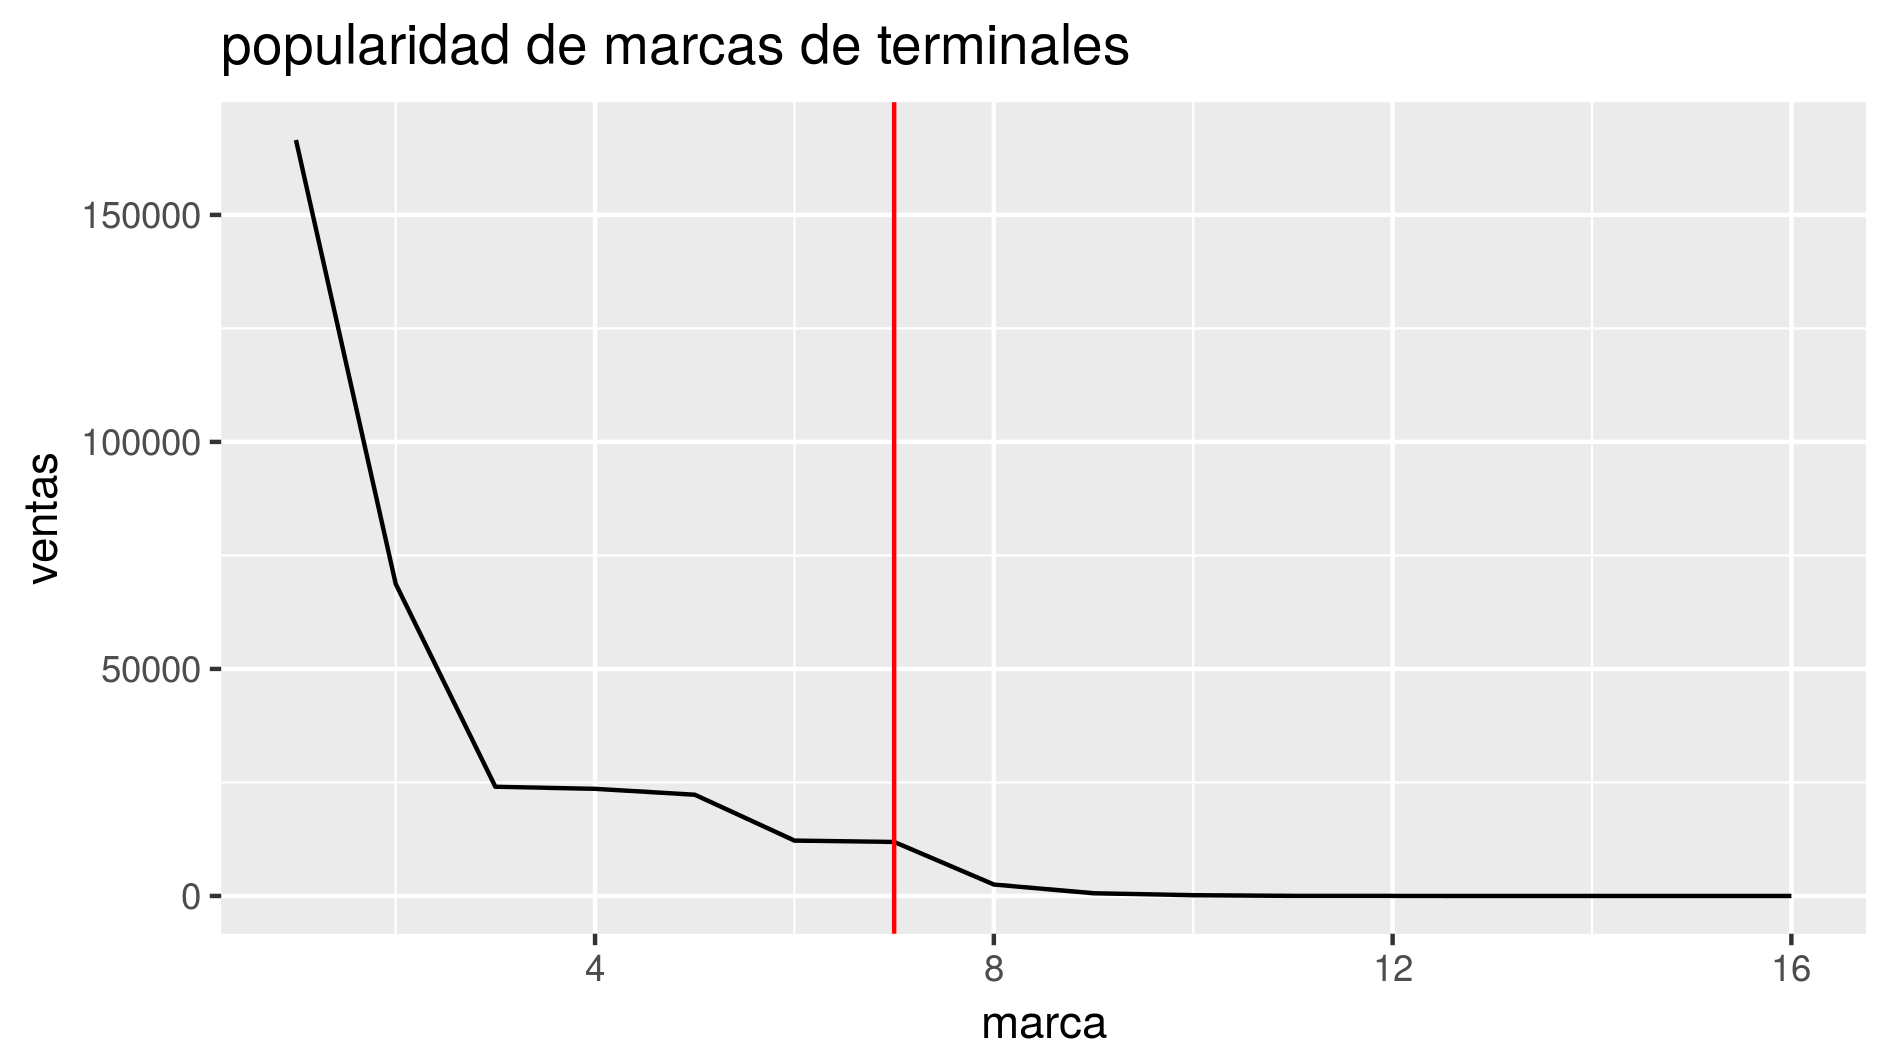
\includegraphics[scale=0.6]{figures/ejemplo.png}
\caption{Cantidad de ventas por marca. Separando con la linea roja las principales marcas del resto.}
\label{fig:marcas}
\end{center}
\end{figure}



\begin{pycode}
from pylab import *

# Define f(t), the desired function to plot
def f(t):
    return cos(2 * pi * t) * exp(-t)

# Generate the points (t_i, y_i) to plot
t = linspace(0, 5, 500)
y = f(t)

# Begin with an empty plot, 5 x 3 inches
clf()
figure(figsize=(5, 3))

# Use TeX fonts
rc("text", usetex=True)

# Generate the plot with annotations
plot(t, y)
title("Damped exponential decay")
text(3, 0.15, r"$y = \cos(2 \pi t) e^{-t}$")
xlabel("time (s)")
ylabel("voltage (mV)")

# Save the plot as a PDF file
savefig("figures/ejemplopy.pdf", bbox_inches="tight")

# Include the plot in the current LaTeX document
#print(r"\begin{center}")
#print(r"\includegraphics[width=0.65\textwidth]{figures/ejemplopy.pdf}")
#print(r"\end{center}")
\end{pycode}

\begin{figure}[bhtp]
\begin{center}
\includegraphics[width=0.65\textwidth]{figures/ejemplopy.pdf}
\caption{Generada on the fly.}
\label{fig:onthefly}
\end{center}
\end{figure}

